\documentclass[12pt,journal]{IEEEtran}

\usepackage{cite}
\usepackage{mathtools}
\usepackage{array}
\usepackage{dblfloatfix}
\usepackage{hyperref}
\usepackage[T1]{fontenc}
\usepackage{inconsolata}
\usepackage{siunitx}

\usepackage{color}
\definecolor{bluekeywords}{rgb}{0.13,0.13,1}
\definecolor{greencomments}{rgb}{0,0.5,0}
\definecolor{redstrings}{rgb}{0.9,0,0}

\usepackage{listings}
\lstset{language=Oz,
	showspaces=false,
	showtabs=false,
	breaklines=true,
	showstringspaces=false,
	breakatwhitespace=true,
	escapeinside={(*@}{@*)},
	commentstyle=\color{greencomments},
	keywordstyle=\color{bluekeywords},
	stringstyle=\color{redstrings},
	basicstyle=\ttfamily,
	tabsize=4
}


\hyphenation{op-tical net-works semi-conduc-tor}

\newcommand{\ntt}{\normalfont\ttfamily}
\newcommand{\fn}[1]{{\protect\ntt#1}}

\begin{document}
\title{Ozploding bozmbs --- Bomberman in Oz}
\author{Alexandre Gobeaux and Gilles Peiffer%
\IEEEcompsocitemizethanks{\IEEEcompsocthanksitem Alexandre Gobeaux -- 42191600\protect\\
E-mail: \href{mailto:alexandre.gobeaux@student.uclouvain.be}{alexandre.gobeaux@student.uclouvain.be}%
\IEEEcompsocthanksitem Gilles Peiffer -- 24321600 \protect\\
E-mail: \href{mailto:gilles.peiffer@student.uclouvain.be}{gilles.peiffer@student.uclouvain.be}}
}

\markboth{Ozploding bozmbs --- Bomberman in Oz}%
{Alexandre Gobeaux and Gilles Peiffer}


\IEEEtitleabstractindextext{%
\begin{abstract}
In this paper, the methodology and design choices behind our implementation of the Bomberman game in Oz are given.
Both the turn-by-turn part of the game controller as its simultaneous part are explained, and an attempt is made to clarify why the authors took certain decisions with regards to how the final product works.
On top of that, an algorithm was implemented in order to control the players' moves, reacting to various messages it receives containing either requests or information about the game.
This was done in at various levels of complexity, building increasingly efficient players.
On top of the mandatory parts of the project, various supplementary features and embellishments are also included in the implementation.

In order to validate our product, interoperability tests were also carried out with both the reference player and other teams' players.
This paper presents a brief summary of the results of these tests.
\end{abstract}
}


\maketitle

\IEEEdisplaynontitleabstractindextext

\section{Introduction}

\IEEEPARstart{B}{omberman} is a famous game involving multiple players, a map with bombs and boxes and several ways to win points and eventually the game.
For this year's project, our task was to implement this game in the Oz programming language.
Implementing the game required writing the code for both the controller, as detailed in Section~\ref{sec:controller}, as well as writing some (not so) rudimentary players, explained in Section~\ref{sec:player}.
To validate our implementation, we conducted interoperability tests with several other groups.
The summaries of these tests are available in Section~\ref{sec:interop}.
Finally, some extensions were implemented, as well as all the mandatory parts.
An exhaustive list of extensions is given in Section~\ref{sec:extensions}.

\section{Controller structure}
\label{sec:controller}
\IEEEPARstart{T}{he} controller in \fn{Main.ozf} can play the game in two modes: turn-by-turn of simultaneously.
We mainly detail the workflow of the turn-by-turn controller, as the simultaneous controller is very similar to this for the main part.

We use the word ``broadcast'' to signify ``send to all players''.

\subsection{Turn-by-turn controller}
When the game starts, the controller starts by creating the window, and creates a list of the players and their ports thanks to \fn{Input.ozf} and \fn{PlayerManager.ozf}.
We then create the map and memorize each player's spawn position, and alert each player of theirs using the \lstinline|assignSpawn(Pos)| message.
Once the GUI is done creating the map, we call the main function of the controller, which starts running the game in turn-by-turn mode, recursively for each round.

This function starts by determining whether the game is over by checking if any of the endgame conditions are met.
The controller then checks if there is any fire that needs to be hidden and explodes bombs that run out of time, broadcasting a \lstinline|bombExploded(Pos)| message if needed.
If any players get hit by the blast, a \lstinline|gotHit(ID Result)| message is sent to them, and information about the death is broadcast to all players.
The controller also remembers who died and checks which boxes got destroyed.
Information about this is broadcast with the appropriate message,
and the endgame conditions are checked again.
Finally, the controller updates the map.
This raises the question of how to indicate bonuses and points laid bare by explosions; in order to handle this case, the controller defines two new tiles: a point tile with value \(5\) and a bonus tile with value \(6\).
When a player moves to one of these, their value is changed back to \(0\), to simulate picking up the reward.

In order to avoid players missing their turn because they got hit by fire before getting a chance to play, we have to respawn the players that died yet still have at least one life left.
We broadcast the spawn information to all players and update the list of positions.
To avoid sending \lstinline|doaction(ID Action)| messages to dead players, the controller maintains a counter (implemented with a stream).
It then checks whether the player's state is \lstinline|on|, skipping the player if not, sending a \lstinline|doaction(ID Action)| message if it is.
The player then determines what its next action will be.
If the action matches \lstinline|move(Pos)|, \fn{Main.ozf} checks if any bonuses or points are picked up, and updates the list of positions.
If the action matches \lstinline|bomb(Pos)|, then the controller tells the GUI to spawn a bomb at the specified position.
It then sends its blast time on the bomb port.
The action is broadcast to all players regardless of the action.
After all this, the function is called recursively and the next turn begins.

\subsection{Simultaneous controller}
For the simultaneous controller, we had to implement random delays in the players, to account for ``thinking time''.
This controller is very similar to the turn-by-turn one.
Conceptually, it works by creating one global thread, common to all players, and then creating a separate thread for every player, sending a \lstinline|doaction(ID Action)| message to each, and waiting for a reply using the \lstinline|Wait| function.
Once this reply is received, it is then sent to a stream on the main thread and handled in a similar way to how it was handled by the turn-by-turn controller.

\section{Player structure}
\label{sec:player}
\subsection{General structure}
\IEEEPARstart{I}{n} order to play the game intelligently, players have to store all relevant information about a game; in order to do this in a clean manner, the authors opted to use record structures, which can easily be modified with the \lstinline|AdjoinList| function.
These records change vary for more advanced players, as they need to store more data about the game in order to make use of their intelligent strategies, but the records always contain at least the following fields:
\begin{itemize}
	\item \lstinline|id|: ID of the player;
	\item \lstinline|state|: state of the player;
	\item \lstinline|lives|: number of remaining lives;
	\item \lstinline|pos|: current position;
	\item \lstinline|sppos|: assigned spawn position;
	\item \lstinline|bombs|: number of bombs owned;
	\item \lstinline|map|: map of the game;
	\item \lstinline|score|: number of points.
\end{itemize}

Players have to respond to different messages they can get from the controller, in the form of a stream of instructions.
In order to handle each of these messages, multiple so-called ``handler functions'' were created, one for each possible instruction.
Most of the messages that a player can receive in its stream are relatively straightforward; in this paper, only the most important instruction, \lstinline|doaction(ID Action)| is explained.

The \lstinline|doaction(ID Action)| message asks the player for its ID and its next action (place a bomb at its current location or move to a neighbouring location).
Multiple players were implemented, with the difference between them lying mainly in the way the ``optimal'' action is computed.
These differences are explained in Section~\ref{sec:playerai}.

\subsection{Decision algorithms}
\label{sec:playerai}
\subsubsection{Basic player}
In our basic random player, \fn{Player001Kardashian.ozf}, the decision algorithm looks like this:
\begin{itemize}
	\item If the player has no bombs left, move to a random neighbour with uniform probability over the acceptable moves.
	\item If the player has bombs left, the player has a \SI{10}{\percent} chance to drop a bomb, and a \SI{90}{\percent} chance to move to a randomly chosen acceptable neighbour.
\end{itemize}

This strategy is not very efficient: the player does not avoid bombs, and does not hunt for points.

\subsubsection{Advanced player}
Our next player, \fn{Player001Tao.ozf}, is slightly more advanced; its decision algorithm tries to avoid standing in dangerous areas, i.e. too close to bombs.
This means that the advanced player has to keep track of where bombs are located.
In order to do this, one must simply add an argument to the \lstinline|summary| record: \lstinline|bomblist|, which stores a list of bombs that are currently on the map.
When the player has to determine its next action, it uses the following algorithm:
\begin{itemize}
	\item If the player has no bombs left, move to the least dangerous acceptable neighbour, where the danger rating of a tile is found by initialising it to zero, and then adding points if the tile is in the blast radius of a bomb (taking into account that walls and boxes stop fire from spreading, as well as the distance from the bomb).
	\item If the player has bombs left, the player has a \SI{10}{\percent} chance to drop a bomb, and a \SI{90}{\percent} chance to move according to the algorithm above.
\end{itemize}

This strategy is more successful than the basic player, and most of the time manages to avoid bombs.
It does not however hunt for points or bonuses, and can make wrong choices when trying to avoid bombs (forcing itself into a dead end, for example).

\subsubsection{Intelligent player}
The intelligent player, \fn{Player001Turing.ozf}, builds further on what the advanced player does, by adding the ability to intelligently search for points and bonuses, with the latter being preferred in most cases.
In order to track where points and bonuses are located, one has to take care of treating the \lstinline|boxRemoved(Pos)| messages.
The algorithm is the following:
\begin{itemize}
	\item If the player has no bombs left, move to the least dangerous acceptable neighbour, where the danger rating of a tile is found by initialising it to zero, and then adding points if the tile is in the blast radius of a bomb (taking into account that walls and boxes stop fire from spreading, as well as the distance from the bomb).
	If multiple neighbours are equally safe, run an iterative deepening depth-first search for points and one for bonuses.
	If possible, the player tries to go for a bonus first, given that the distance to the next bonus is not too big compared to the distance to the next point\footnote{Heuristically, we found \(d_{\textnormal{bon}} > 3d_{\textnormal{pt}}\) to be a good cutoff value.}.
	If there is a point target and no bonuses, the player moves towards it on the shortest path.
	Finally, if there are no special targets, the player chooses a random neighbour from the safe options.
	\item If the player has bombs left, it tries to place a bomb given that it is next to a box (in order to lay bare its content).
	Otherwise, it moves towards a position according to the algorithm above.
\end{itemize}

This strategy works very well, and won every single interoperability game it competed in.

\subsubsection{Competitive player}
The intelligent player, \fn{Player001Dijkstra.ozf}, builds further on what the intelligent player does, by adding the ability to intelligently search for points and bonuses, with the latter being preferred in most cases.
In order to track where points and bonuses are located, one has to take care of treating the \lstinline|boxRemoved(Pos)| messages.
The algorithm is the following:
\begin{itemize}
	\item If the player has no bombs left, move to the least dangerous acceptable neighbour, where the danger rating of a tile is found by initialising it to zero, and then adding points if the tile is in the blast radius of a bomb (taking into account that walls and boxes stop fire from spreading, as well as the distance from the bomb).
	If multiple neighbours are equally safe, run an iterative deepening depth-first search for points, for bonuses and for boxes of both types.
	The bomber first tries to hunt for these special targets, prioritizing bonuses, then points, then boxes in the same respective order.
	Finally, if there are no special targets, the player chooses a random neighbour from the safe options.
	\item If the player has bombs left, it tries to place a bomb given that it is next to a box (in order to lay bare its content).
	Otherwise, it moves towards a position according to the algorithm above.
\end{itemize}

This player is similar to the intelligent player, but avoids the possibility of the game ``dying out'' on bigger maps.

\subsection{Simultaneous players}
In order to be able to play the game in simultaneous mode, we had to implement a thinking delay in the players when deciding on their next action.
The code for that is of the form
\begin{lstlisting}
if Input.isTurnByTurn then
	% Decide next move.
else
	thread
		% Random think delay.
		% Decide next move.
	end
end
\end{lstlisting}

\section{Interoperability}
\label{sec:interop}
\IEEEPARstart{I}{n} order to validate our implementation, we carried out interoperability tests with various groups.
These tests helped us to identify misunderstandings in the project specification, as well as find some tricky bugs.
Where necessary, players were renamed to conform to the naming guideline specified in the project statement.

\subsection{Group 0 -- Maudoux, Verhaeghe}
\subsubsection{\fn{Player000bomber.ozf}}
Testing for interoperability with the default player helped us get started, and helped improve our algorithms.
All our players work with the default player, in either mode.

\subsection{Group 7 -- Bousselmi, Zarza Davila}
\subsubsection{\fn{Player007Scared.ozf}}
With this group, the interoperability test was repeated twice, playing in the simultaneous mode, on each controller and with \fn{Player001Turing.ozf}.
While testing, we found their player's behavior, while erratic, to be correct.
Our player performed quite well, winning both rounds comfortably.
Other than that, nothing really worth mentioning happened; both players and controllers seemed correct.

\subsection{Group 9 -- Thibaut, Tran}
\subsubsection{\fn{Player009defense.ozf}}
This group's player was tested in the simultaneous mode, against both of our more advanced players.
This gave us another good indication that our implementations conform to the requirements laid out in the project statement.
\subsubsection{\fn{Player009notsafedefense.ozf}}
Like this group's other player, this interoperability test went well, with both players doing what they were supposed to.

\subsection{Group 10 -- Nguyen, Verbois}
\subsubsection{\fn{Player010IA2.ozf}}
This player was tested in the simultaneous game mode on our computer and in the turn-by-turn mode on theirs, against \fn{Player001Turing.ozf}.
Our AI clearly proved superior, but both players performed as expected and respected the project requirements.

\subsection{Group 13 -- De Vogeleer, Diels}
\subsubsection{\fn{Player013smart.ozf}}
Both advanced players were tested with this implementation, yielding correct results both in turn-by-turn mode and simultaneous mode.

\subsection{Group 17 -- Clément, Moueddene}
\subsubsection{\fn{Player017advanced.ozf}}
In this test, each group tested one mode, on the default map and with \fn{Player001Turing.ozf} as the player's opponent.
The latter won both games, and no problems were found with the controllers or players.

\subsection{Group 38 -- de Keersmaeker, Gérard}
\subsubsection{\fn{Player038Luigi.ozf}}
Testing our implementation's interoperability with this group proved fruitful: while testing in the simultaneous mode, with our own \fn{Player001Turing.ozf} playing against itself, on the same side of the default map, they found one of them suffers an interesting decrease in performance.
Even with this decrease, our players still won the game, but this helped us further improve the player.
Their player, while not as performant, performed as expected both in simultaneous as in turn-by-turn mode.

\subsection{Group 55 -- Mulders, Semerikova}
\subsubsection{\fn{Player055Random.ozf}}
While trying for interoperability with this group, we were reminded that our player is not allowed to place two bombs on the same tile.
In order to fix this mistake, we had to rework the way the list of bombs is kept.
Thinking about this also helped us to solve another issue we had when playing simultaneously; with the new design, our implementation was no longer specifically tailored to a certain game mode, i.e. turn-by-turn.
Another error we found is that the advanced players did not always bind an ID when returning an Action.
Since our \fn{Main.ozf} was very robust and did not actually need these values as they were being kept track of, the error never showed on our own computers.

Another issue we ran into while testing our players with this group was that after some rounds, our player would stop planting bombs, despite being under the right circumstances to do so.
When investigating the code, this came down to a mismatch in specifications between the initialisation of the list of bombs and the \lstinline|case| statement trying to access it.

\subsubsection{\fn{Player055Survivor.ozf}}
This test, on both controllers and with \fn{Player001Kardashian} as the opponent, worked well and allowed us to verify the correctness of our player.
The game was played in turn-by-turn mode on their machine, and simultaneous mode on ours.

\subsubsection{\fn{Player005Clever.ozf}}
As we were playing a game against their advanced player, we suggested a different, more efficient approach.
There were no bugs with their player or their controller, as far as we could see.

\subsection{Group 100 -- Gevorgyan, Navarre}
\subsubsection{Player100JonSnow.ozf}
This player was tested in both modes against both of our more advanced players.
\fn{Player001Turing.ozf} proved to be the better player, but this test led to some interesting discussions regarding the optimal way to search for points in a graph (comparing breadth-first search to iterative deepening depth-first search).

\subsubsection{\fn{Player100advanced.ozf}}
Using both controllers, this player was tested against both \fn{Player001Tao.ozf} and \fn{Player001Turing.ozf}.
The latter won its games convincingly, and all four players worked perfectly on both controllers, in every mode.

\subsection{Group 105 -- Maréchal, Martin}
\subsubsection{UniMate interoperability platform}
Our player \fn{Player001Turing.ozf} was tested on the interoperability platform on a variety of maps.
While its score there was limited by the fact that our player is rather trigger-happy, this still showed that its algorithms are rather strong.

\section{Extensions and optional parts}
\label{sec:extensions}
\IEEEPARstart{S}{ome} of the proposed extensions and improvements were implemented, and the authors added some of their own:
\begin{itemize}
	\item As explained in Section~\ref{sec:playerai}, one of our players,
	\fn{Player001Turing.ozf}, uses a fairly advanced algorithm to determine its next action.
	\item The GUI has been embellished to resemble the user interface of the Minecraft game.
	\begin{figure}[!hbtp]
		\centering
		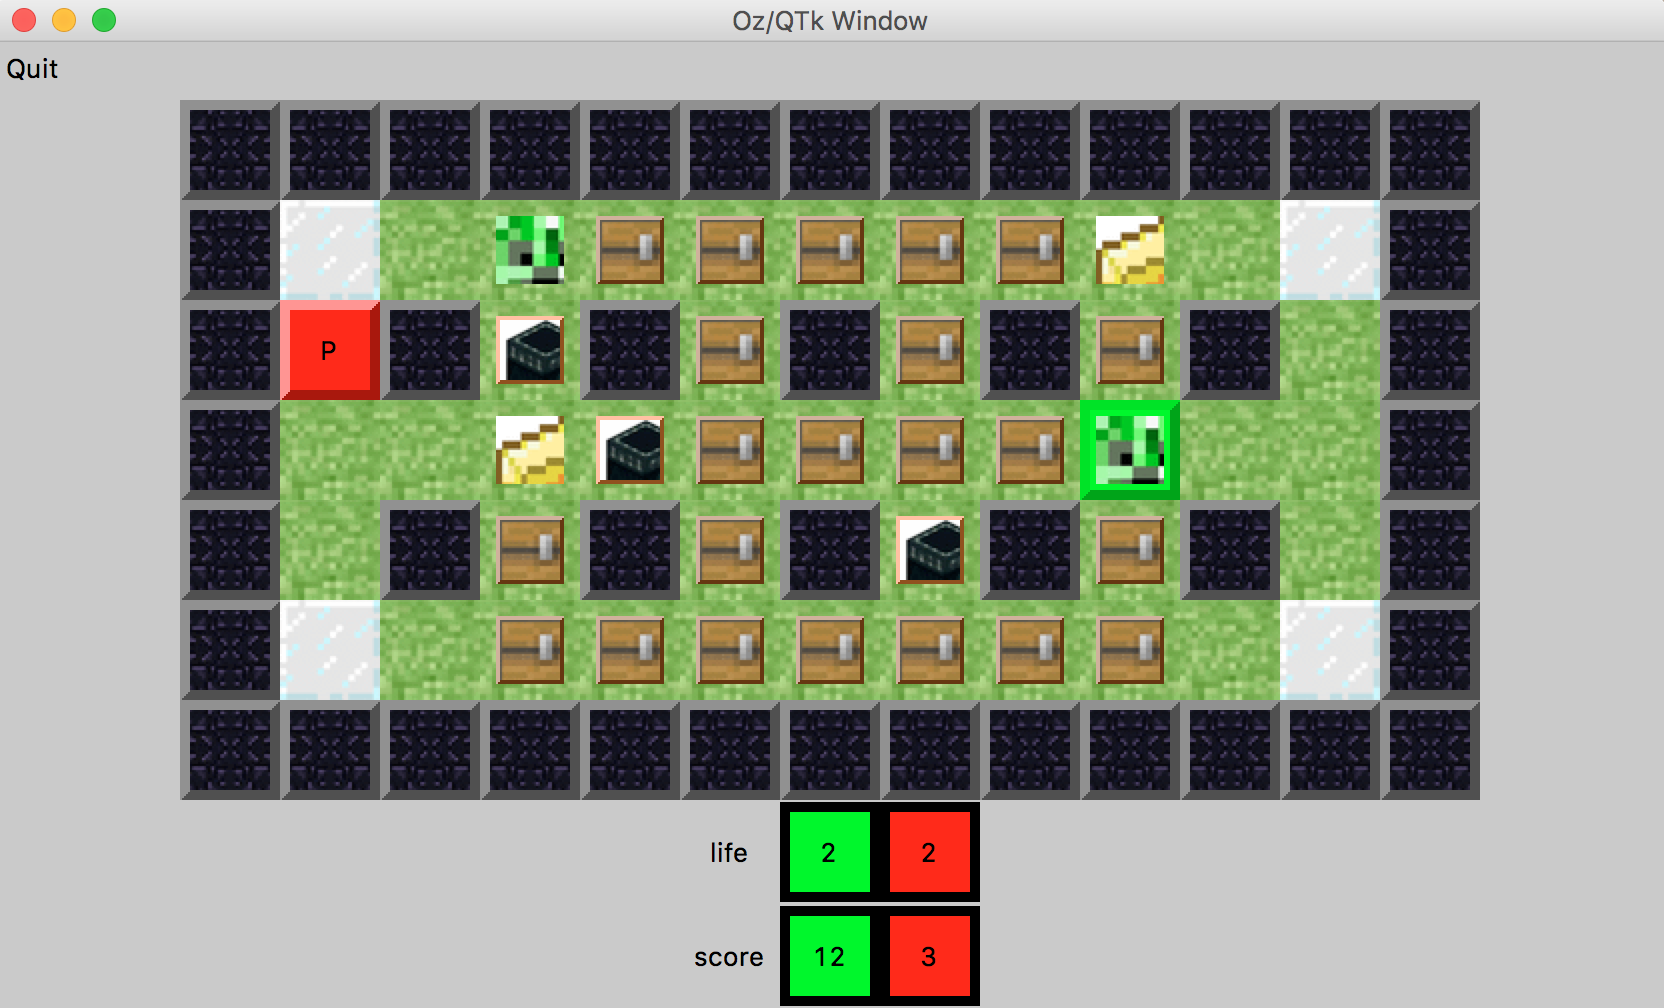
\includegraphics[width=\columnwidth]{gui.png}
		\caption{A Minecraft-based user interface.}
		\label{fig:gui}
	\end{figure}
	\item The synchronization between the GUI and the controller has been automated, to avoid the game starting while the GUI is still loading.
	\item Other options were added for the bonus, such as a malus of \(1\) point.
	Our players are also able to deal with the \lstinline|add(life, 1)| bonus.
	\item More interoperability tests were included than required, so as to make sure our implementations are correct.
\end{itemize}

\section{Conclusion}
\IEEEPARstart{W}{orking} on this project has helped us to better understand how to work with the multiple programming paradigms taught during the course.
It introduced us to working with artificial intelligence on the players and algorithms.
While the Oz language is arguably not the best choice for these kinds of tasks, some of its features such as records proved a great asset in writing clean, efficient and scalable code.
Adding a simultaneous mode brought concurrency into the mix, which proved to be easier than we previously thought once we understood how to proceed with it.
Finally, the opportunity to add extensions allowed us to let go of our creativity and try to make something visually appealing, while adding features to the game at the same time.

\end{document}


